\documentclass[a4paper,10pt]{article}
\usepackage{fullpage}
\usepackage[british]{babel}
\usepackage[T1]{fontenc}
\usepackage{amsmath}
\usepackage{epstopdf}
\usepackage{amssymb}
\usepackage[T1]{fontenc}
\usepackage[utf8]{inputenc}
%\usepackage{amsthm} \newtheorem{theorem}{Theorem}
\usepackage{color}
\usepackage{float}
%\usepackage{todonotes}
\usepackage{caption}
\DeclareCaptionFont{white}{\color{white}}
\DeclareCaptionFormat{listing}{\colorbox{gray}{\parbox{\textwidth}{#1#2#3}}}
\captionsetup[lstlisting]{format=listing,labelfont=white,textfont=white}

\usepackage{alltt}
\usepackage{listings}
 \usepackage{aeguill}
\usepackage{dsfont}
%\usepackage{algorithm}
%\usepackage[noend]{algorithm2e}
%\usepackage{algorithmicx}
\usepackage{subfig}
\lstset{% parameters for all code listings
language=ada,
frame=none,
basicstyle=\small, % nothing smaller than \footnotesize, please
tabsize=2,
%numbers=left,
 framexleftmargin=2em, % extend frame to include line numbers
xrightmargin=2em, % extra space to fit 79 characters
breaklines=true,
breakatwhitespace=true,
prebreak={/},
captionpos=b,
columns=fullflexible,
escapeinside={\#*}{\^^M}
}


% Alter some LaTeX defaults for better treatment of figures:
    % See p.105 of "TeX Unbound" for suggested values.
    % See pp. 199-200 of Lamport's "LaTeX" book for details.
    % General parameters, for ALL pages:
    \renewcommand{\topfraction}{0.9}	% max fraction of floats at top
    \renewcommand{\bottomfraction}{0.8}	% max fraction of floats at bottom
    % Parameters for TEXT pages (not float pages):
    \setcounter{topnumber}{2}
    \setcounter{bottomnumber}{2}
    \setcounter{totalnumber}{4} % 2 may work better
    \setcounter{dbltopnumber}{2} % for 2-column pages
    \renewcommand{\dbltopfraction}{0.9}	% fit big float above 2-col. text
    \renewcommand{\textfraction}{0.07}	% allow minimal text w. figs
    % Parameters for FLOAT pages (not text pages):
    \renewcommand{\floatpagefraction}{0.7}	% require fuller float pages
% N.B.: floatpagefraction MUST be less than topfraction !!
    \renewcommand{\dblfloatpagefraction}{0.7}	% require fuller float pages

% remember to use [htp] or [htpb] for placement


\usepackage{fancyvrb}
%\DefineVerbatimEnvironment{code}{Verbatim}{fontsize=\small}
%\DefineVerbatimEnvironment{example}{Verbatim}{fontsize=\small}

\newcommand{\keywords}[1]{\par\addvspace\baselineskip
\noindent\keywordname\enspace\ignorespaces#1}


\usepackage{tikz} \usetikzlibrary{trees}
\usepackage{hyperref} % should always be the last package

% useful colours (use sparingly!):
\newcommand{\blue}[1]{{\color{blue}#1}}
\newcommand{\green}[1]{{\color{green}#1}}
\newcommand{\red}[1]{{\color{red}#1}}

% useful wrappers for algorithmic/Python notation:
\newcommand{\length}[1]{\text{len}(#1)}
\newcommand{\twodots}{\mathinner{\ldotp\ldotp}} % taken from clrscode3e.sty
\newcommand{\Oh}[1]{\mathcal{O}\left(#1\right)}

% useful (wrappers for) math symbols:
\newcommand{\Cardinality}[1]{\left\lvert#1\right\rvert}
%\newcommand{\Cardinality}[1]{\##1}
\newcommand{\Ceiling}[1]{\left\lceil#1\right\rceil}
\newcommand{\Floor}[1]{\left\lfloor#1\right\rfloor}
\newcommand{\Iff}{\Leftrightarrow}
\newcommand{\Implies}{\Rightarrow}
\newcommand{\Intersect}{\cap}
\newcommand{\Sequence}[1]{\left[#1\right]}
\newcommand{\Set}[1]{\left\{#1\right\}}
\newcommand{\SetComp}[2]{\Set{#1\SuchThat#2}}
\newcommand{\SuchThat}{\mid}
\newcommand{\Tuple}[1]{\langle#1\rangle}
\newcommand{\Union}{\cup}
\usetikzlibrary{positioning,shapes,shadows,arrows}

\newcommand{\answer}{\textbf{Answer: }}
\newcommand{\query}[1]{\lstinline{#1}}

\usepackage{url}


\pagestyle{empty}

\title{Realtime Systems - Fall 2013 \\ \textbf{Lab 4 Report}}

\author{Bjorn Forsberg, Jonathan Sharyari, Daniel Tibbing}

\begin{document}

\maketitle

\section*{Part 1: Verification Warm-Up}

The three automatons were modelled as specified, and verified in UPPAAL. The questions and their corresponding answers follow:

\begin{itemize}
  \item \emph{Can the value of the variable i become strictly greater than 200?}
    
    \answer The property is \emph{not} satisfied. The following query was used: 

    \query{E<> i > 200}
  \item \emph{Is it true that no matter what happens (always) is the value of i smaller than or equal to 100?}
    
    \answer The property is satisfied. The following query was used:

    \query{A[] i <= 100}
  \item \emph{Is it true that no matter what happens (always) is the value of i strictly smaller than 100?}
    
    \answer The property is \emph{not} satisfied. The following query was used:

    \query{A[] i < 100}
  \item \emph{Can the value of the variable i be equal to 37?}
    
    \answer The property is satisfied. The following query was used:

    \query{E<> i == 37}
  \item \emph{Is it true that no matter what happens (always) is the value of i greater than or equal to 0?}
    
    \answer The property is \emph{not} satisfied. The following query was used:

    \query{A[] i >= 200}
\end{itemize}

\section*{Part 2: Scheduling}

In this part, we scheduled a number of processes on two processors. The processor template was given in the assignment, the Job template can be seen in Figure \ref{img:part2extendedJob}.

\begin{figure}[h]
  \center
  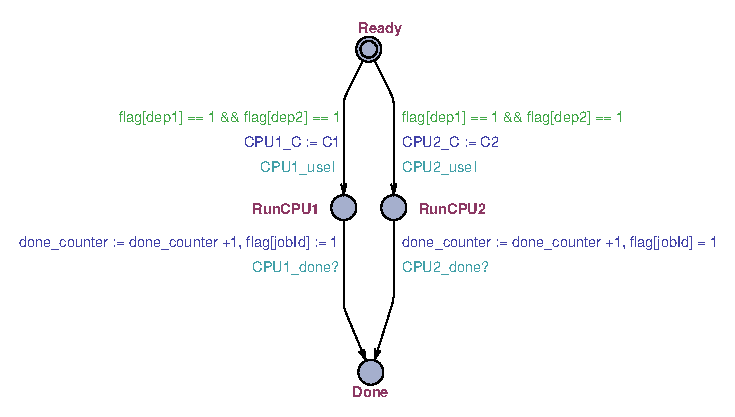
\includegraphics{Part2Extended}
  \caption{The Job template for Part 2.}
  \label{img:part2extendedJob}
\end{figure}

The Job template consists of four states (Ready, RunCPU1, RunCPU2, Done). When we are in the ready state we can select which processor to run the job on, given that the dependencies are met. The dependency check is done against an array that keeps track of which jobs have finished. If there are no dependencies, the dependency index is set to 0 (jobs are indexed from 1), which is always 1 (true).

If the dependencies are met, we set the execution time of the processor in question to the execution time of the job on that processor. To signal the processor to start execution, synchronization is used. This moves the job to the RunCPU\# (\# = 1,2) state.

Once the execution is finished, we receive the CPU\#\_done signal and increase the done\_counter (number of jobs finished) with 1, representing the finished job. We also set the done flag in the dependency vector of the current task to 1 (true), which will allow jobs that depend on our job to start. This moves the job to the Done state.

\subsection*{Response time analysis}

To finish off this part of the lab we run our system with the jobs described in Figure \ref{tab:part2jobtable}. The goal was to calculate the shortest execution time for the tasks which was done and verified as follows.

\begin{figure}[h]
\center
\begin{tabular}{l | l | l | l}
  \hline
  Job id & $C_1$ & $C_2$ & Waits for \\
  \hline
  A & 1 & 2 & - \\
  B & 4 & 2 & - \\
  C & 5 & 5 & A \\
  D & 2 & 4 & A, B \\
  E & 3 & 7 & B \\
  F & 7 & 8 & C \\
  G & 1 & 1 & C, D \\
  H & 5 & 2 & G, E \\
  I & 3 & 1 & E \\
  \hline
\end{tabular}
\caption{The job table for Part 2.}
\label{tab:part2jobtable}
\end{figure}


To get the shortest execution time we ran the query:

\begin{itemize}
\item[]\query{E<> done\_counter == 9}
\end{itemize}

This gives us the fastest response time of the tasks, which was 14. To verify that this is indeed the optimal we used the following query:

\begin{itemize}
\item[] \query{E<> (done\_counter == 9) and (y < 14)}
\end{itemize}

This query was not satisfied, which means that there is no schedule that finishes the task faster than the calculated 14 tu (time units).

If we had not included the first query, the verification would be complete by also verifying that 14 is indeed a plausible execution time. This was done using the query:

\begin{itemize}
\item[] \query{E<> (done\_counter == 9) and (y == 14)}
\end{itemize}

The query was satisfied and we can therefore with certainty say that 14 is indeed the fastest response time of this system.


\section*{Part 3: Deadlock}

The last part of the Lab consisted of modelling the Producer-Consumer program from Lab 1. The model for the Producer was given in the assignment. The Consumer and Buffer models were implemented by us and can be seen in Figure \ref{img:part3consumer} and Figure \ref{img:part3buffer} respectively.

\begin{figure}[h]
  \center
  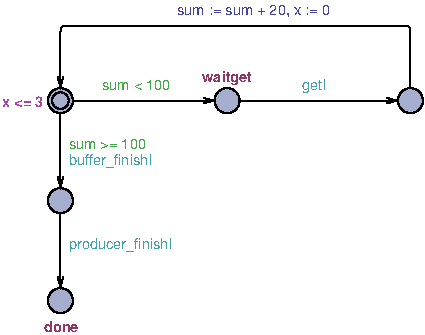
\includegraphics{Part3Consumer.pdf}
  \caption{The first Consumer template for Part 3.}
  \label{img:part3consumer}
\end{figure}

\begin{figure}[h]
  \center
  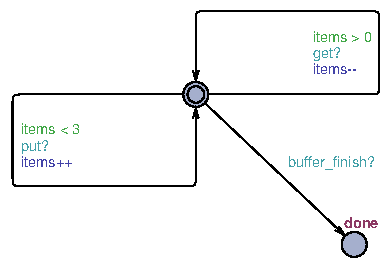
\includegraphics{Part3BufferFixed.pdf}
  \caption{The first Buffer template for Part 3.}
  \label{img:part3buffer}
\end{figure}

This model included deadlocks, which we identified using UPPAAL. Since the Done states in the templates are by definition deadlocked states these had to be excluded since this is the expected behaviour of the program. UPPAAL includes the macro \texttt{deadlock} to use in queries, but to ignore the done states the following query was used:

\begin{itemize}
  \item[] \query{A[] (not deadlock)  or (Consumer.done and Producer.done and Buffer.done)}
\end{itemize}

This query allowed us to identify a real deadlock in the program, namely the case when we finish the Buffer before finishing the Producer. This means that the Producer will deadlock in the \emph{waitput} state, since there is no buffer to write to. The solution to this is to change the order in which we send the finish commands, to make sure that the Producer finishes before the Buffer.

In a perfect world, this would be the end of deadlocks in the system, however, another deadlock exists in the program.

The second deadlock is in the state where the Consumer has consumed enough values to send the finish signals to the Producer and the Buffer, but the Producer has already chosen to try to write to the Buffer. Since the Consumer has already reached its maximum value it will not read any more items from the buffer, and the Consumer will never be able to write. This potential deadlock can be removed by removing the unnecessary \emph{waitput} state (from which we do not accept the finish signal) to make sure that we are able to receive the finish signal in all cases that we are not in the process of writing items to the Buffer.

In the same fashion, while it isn't a potential deadlock situation, the \emph{waitget} state in the Consumer is also superfluous and was also removed to keep the appearance of the templates alike. This is however only for esthetical reasons.

The final Producer, Consumer and Buffer templates can be seen in Figure \ref{img:part3producerFixed}, Figure \ref{img:part3consumerFixed} and Figure \ref{img:part3bufferFixed} respectively.

\begin{figure}[h]
  \center
  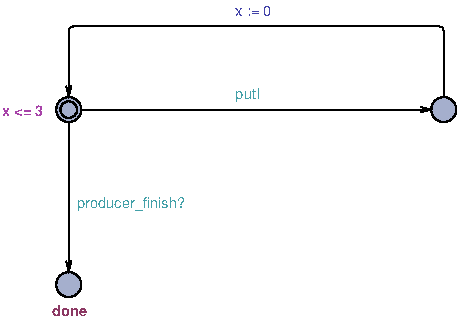
\includegraphics{Part3ProducerFixed.pdf}
  \caption{The final Producer template for Part 3.}
  \label{img:part3producerFixed}
\end{figure}

\begin{figure}[h]
  \center
  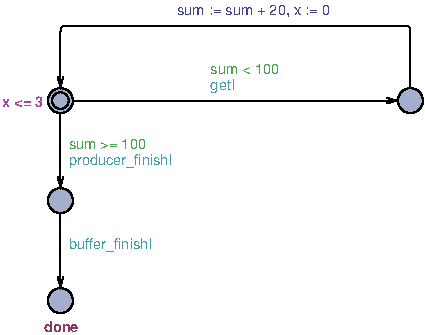
\includegraphics{Part3ConsumerFixed.pdf}
  \caption{The final Consumer template for Part 3.}
  \label{img:part3consumerFixed}
\end{figure}

\begin{figure}[h]
  \center
  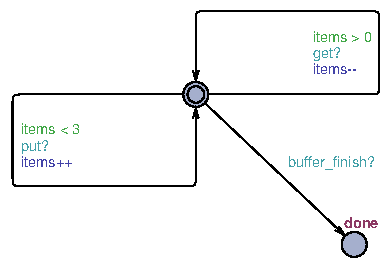
\includegraphics{Part3BufferFixed.pdf}
  \caption{The final Buffer template for Part 3.}
  \label{img:part3bufferFixed}
\end{figure}

The verification queries described above are now satisfied.

\end{document}
